\documentclass[9pt,twocolumn,twoside]{styles/osajnl}
\usepackage{fancyvrb}
\journal{i524} 

\title{MongoDB}

\author[1,*]{Nandita Sathe}

\affil[1]{School of Informatics and Computing, Bloomington, IN 47408, U.S.A.}

\affil[*]{Corresponding author: nsathe@iu.edu}

\dates{paper-1, \today}

\ociscodes{Cloud, I524}

% replace this with your url in github/gitlab
\doi{\url{https://github.com/nsathe/sp17-i524/blob/master/paper1/S17-IO-3017/report.pdf}}


\begin{abstract}
The data that Internet and various gadgets generate today has increased manifold than yesterday. This data is voluminous, complex and un-structured. This arises the need of having a flexible, scalable, and robust database that will not only store this data but also provide it as required in lightening speed. Many NoSQL databases came into existence. Out of them, MongoDB is the fastest-growing database ecosystem. It is the next-generation database that helps businesses transform their industries by harnessing the power of data.\newline
\end{abstract}

\setboolean{displaycopyright}{true}

\begin{document}

\maketitle

\section{Introduction}

MongoDB is a non-RDBMS key-value data store. The data to be stored does not necessarily have to follow a fixed schema. In relational database data is stored primarily in tables, whereas in MongoDB data is stored in collections which act as container for a Document. A Document can be compared to a row of a table. The data in MongoDB Document is stored in JSON array like data structure. The database also supports large volume of data storage and offers very high data insert speed due to its schema-less design. The database system can be used for Big Data applications where volume of incoming data is huge and of varied structure.

\section{Infrastructure and Performance Considerations}

Capacity planning is the most important thing when deciding about production deployments in every environment. Applications may change their percentage of writes versus reads over time. An increase in users typically lead to more queries and a larger working set.

System performance and capacity planning are two important topics that should be addressed in any deployment. The planning should involve establishing baselines on data volume, system load, performance (throughput and latency), and capacity utilization. These baselines should reflect the workloads you expect the database to perform in production, and they should be revisited periodically as the number of users, application features, performance SLA, or other factors change. Baselines will help you understand when the system is operating as designed, and when issues begin to emerge that may affect the quality of the user experience or other factors critical to the system. The following section discusses key deployment considerations, including hardware, scaling and HA. The section also discusses what you need to monitor to maintain optimum system performance.

\subsection{Determine working set size}

\cite{www-mongo4} When prioritizing hardware budget for MongoDB deployments, RAM should be at or near the top of the list.

MongoDB makes extensive use of RAM for low latency database operations. In MongoDB, all data is read and manipulated through memory-mapped files. Reading data from memory is measured in nanoseconds and reading data from disk is measured in milliseconds; and so reading from memory is approximately 100,000 times faster than reading from disk.

The set of data and indexes that are accessed most frequently during normal operations is called the working set, which ideally should fit in RAM. It may be the case that the working set represents a fraction of the entire database, such as applications where data related to recent events or popular products is accessed most commonly.

Page faults occur when MongoDB attempts to access data that has not been loaded in RAM. If there is free memory then the operating system will locate the page on disk and load it into memory directly. However, if there is no free memory the operating system must write a page that is in memory to disk and then read the requested page into memory. This process will be slower than accessing data that is already in memory.

Some operations may inadvertently purge a large percentage of the working set from memory, which adversely affects performance. For example, a query that scans all Documents in the database, where the database is larger than the RAM on the server, will cause documents to be read into memory and the working set to be written out to disk. Ensuring you have defined appropriate index coverage for your queries during the schema design phase of the project will minimize the risk of this happening. The MongoDB {\bfseries explain} method can be used to provide information on your query plan and indexes used.

A useful output resulted from the MongoDB’s {\bfseries serverStatus} command is a workingSet document that provides an estimated size of the MongoDB instance’s working set. Database Administration team can track the number of pages accessed by the instance over a given period, and the elapsed time from the oldest to newest document in the working set. By tracking these metrics, it is possible to detect when the working set is approaching current RAM limits and proactively take action to ensure the system is scaled.

MongoDB Management Service and {\bfseries mongostat} command help to monitor memory usage and are discussed in detail below.

\subsection {Storage and Disk I/O}

While your MongoDB system should be designed so that its working set fits in memory, disk I/O is still a key performance consideration. MongoDB regularly flushes writes to disk and commits to the journal, so under heavy write load, the underlying disk subsystem may become overwhelmed. The {\bfseries iostat} command can be used to show high disk utilization and excessive queuing for writes.

\subsection {CPU Selection – Speed or Cores?}

MongoDB performance is typically not CPU-bound. As MongoDB rarely encounters workloads and is able to leverage large numbers of cores, it is preferable to have servers with faster clock speeds than numerous cores with slower clock speeds.

\subsection {Scaling your Database}

MongoDB provides horizontal scale-out for databases using a technique called sharding. Sharding distributes data across multiple physical partitions called shards. Sharding allows MongoDB deployments to address the hardware limitations of a single server, such as bottlenecks in RAM or disk I/O, without adding complexity to the application.

Figure \ref{fig:figure1} shows scaling of database.

\begin{figure}[htbp]
\centering
\fbox{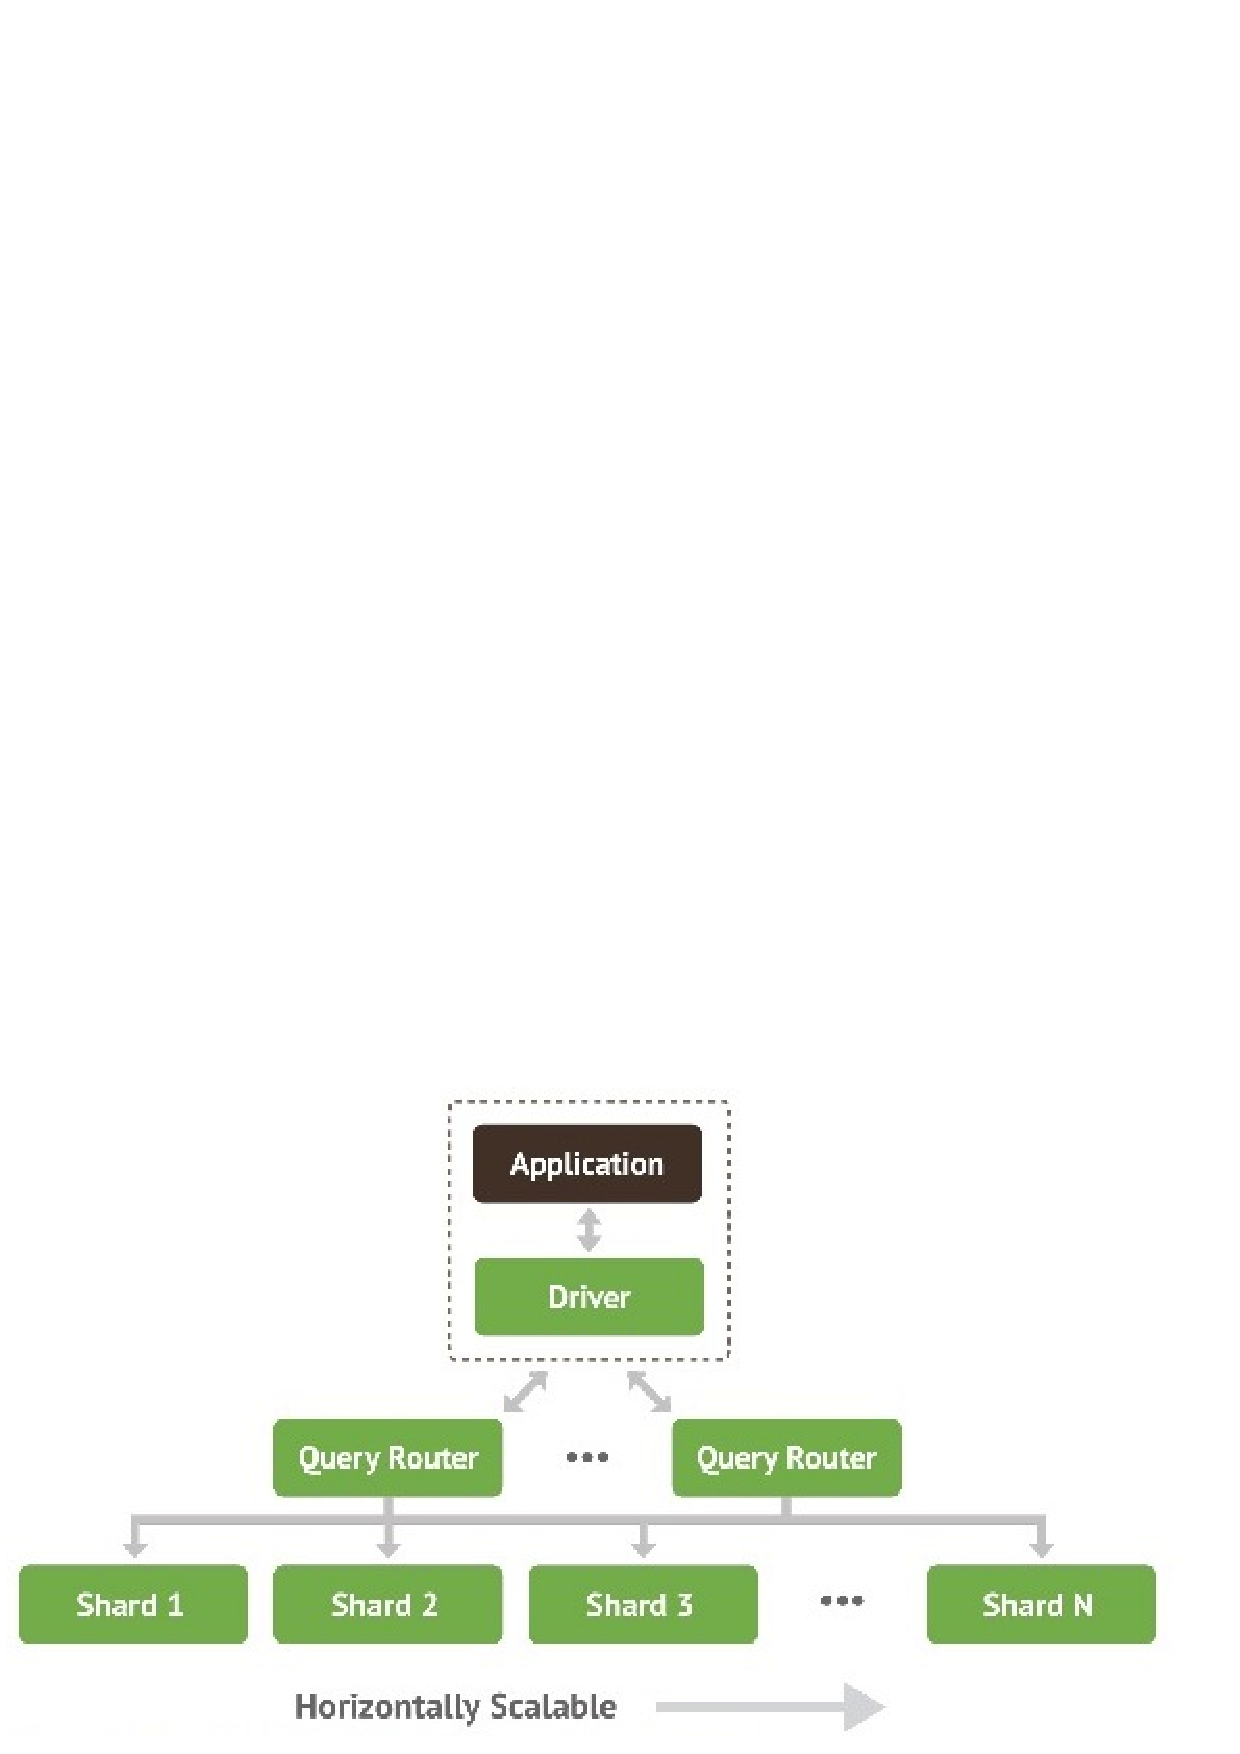
\includegraphics[width=\linewidth]{images/figure1}}
\caption{MongoDB database scaling.}
\label{fig:figure1}
\end{figure}

\subsection {MongoDB Auto-Sharding with Application Transparency}

It is far easier to implement sharding before the resources of the system become limited. That is why capacity planning and proactive monitoring are important elements in successfully scaling the application

Users should consider deploying a sharded MongoDB cluster in the following situations:

{\bfseries RAM Limitation:} The size of the system’s active working set will soon exceed the capacity of the maximum amount of RAM in the system.

{\bfseries Disk I/O Limitation:} The system has a large amount of write activity, and the operating system cannot write data fast enough to meet demand; and/or I/O bandwidth limits how fast the writes can be flushed to disk.

{\bfseries Storage Limitation:} The data set approaches or exceeds the storage capacity of a single node in the system.

One of the goals of sharding is to uniformly distribute data across multiple servers. If the utilization of server resources is not approximately equal there may be an underlying issue that is problematic for the deployment. For example, a poorly selected shard key can result in uneven data distribution. In this case, most if not all of the queries will be directed to the single mongodb that is managing the data.
Furthermore, MongoDB may be attempting to redistribute the documents to achieve a more ideal balance across the servers. While redistribution will eventually result in a more desirable distribution of documents, there is substantial work associated with re-balancing the data and this activity itself may interfere with achieving the desired performance SLA.
By running {\bfseries db.currentOp()} you will be able to determine what work is currently being performed by the cluster, including re-balancing of documents across the shards.
In order to ensure data is evenly distributed across all shards in a cluster, it is important to select a good shard key.

\subsection {High Availability with MongoDB Replica Sets}

MongoDB uses its native replication to maintain multiple copies of data across replica sets. Replica sets help prevent downtime by detecting failures (server, network, OS or database) and automatically initiating failover. It is recommended that all MongoDB deployments should be configured with replication.

Figure \ref{fig:figure2} shows replica sets maintained by MongoDB.

\begin{figure}[htbp]
\centering
\fbox{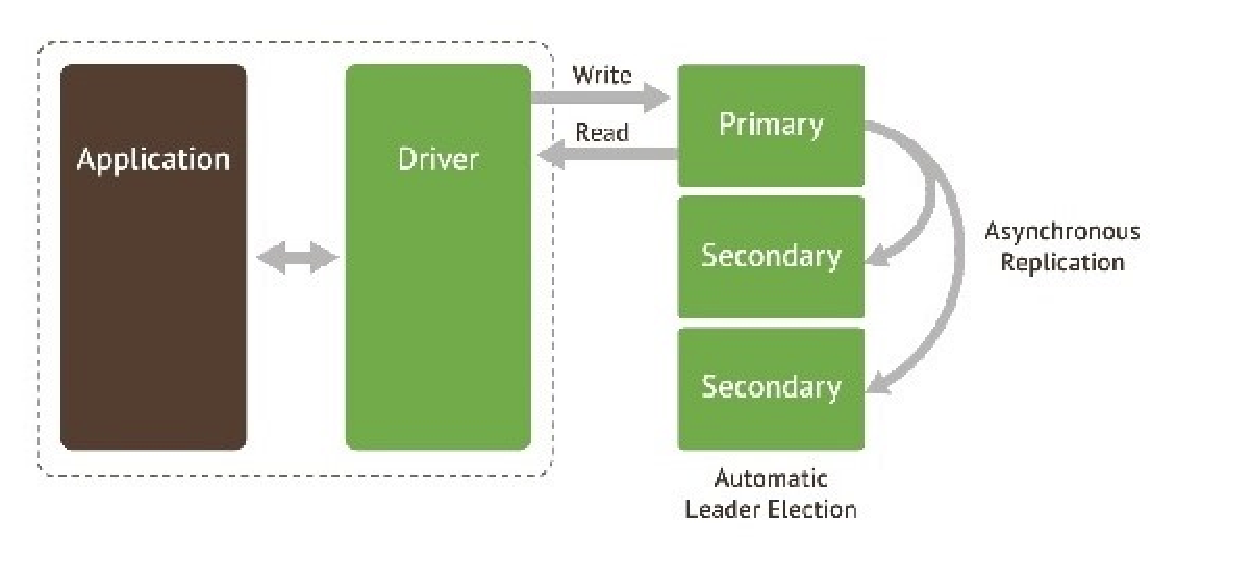
\includegraphics[width=\linewidth]{images/figure2}}
\caption{MongoDB replica sets.}
\label{fig:figure2}
\end{figure}

\section{Features}

These are main features of MongoDB.\cite{www-mongo11}
\begin{itemize}
\item General purpose database, almost as fast as the key:value NoSQL type.

\item High availability.
\item Scalability: (from a standalone server to distributed architectures of huge clusters). This allows us to shard our database transparently across all our shards. This increases the performance of our data processing.
\item Aggregation: batch data processing and aggregate calculations using native MongoDB operations.
\item Load Balancing: automatic data movement across different shards for load balancing. The balancer decides when to migrate the data and the destination Shard, so they are evenly distributed among all servers in the cluster. Each shard stores the data for a selected range of our collection according to a partition key.
\item Native Replication: syncing data across all the servers at the replica set.
\item Security: authentication, authorization, etc.
\item Advanced users management.
\item Automatic failover: automatic election of a new primary when it has gone down.
\item Zero downtime upgrades.
\item There are no bottlenecks processing large volumes of data.
\item MongoDB uses JSON objects to store and transmit information. 
\item We can do queries and geospatial operations in 2D and 3D.
\item We can utilize Map-Reduce for information processing using JavaScript functions at the server side.
\item JavaScript execution: Ability to store JavaScript functions on the server for queries and aggregation functions
\item MongoDB Management Service. (MMS) is a powerful web tool that allows us tracking our databases and our machines and also backing up our data.
\item Monitoring:
\begin{enumerate}
    \item MMS tracks the database and hardware metrics for managing a MongoDB deployment
    \item Performance is visualized in a rich web console to help you optimize your deployment
    \item Custom alerts: Discover issues before your MongoDB instance will be affected
\end{enumerate}
\item Backup
\begin {enumerate}
    \item Continuous backup with point-in-time recovery of replica sets and sharded clusters
    \item Multiple copies of every backup are archived across data centers (geographically distributed and fault-tolerant)
\end{enumerate}
\end{itemize}

\section{MongoDB for BigData Analytics}

At the top level there are 3 Vs that define BigData \cite{www-mongo1}

{\bfseries Volume:}

MongoDB supports storage of high volume of data which is complex in nature. The system is designed in such a way that for larger data loads the data can be distributed across multiple clusters, providing new levels of availability and scalability with no downtime.

{\bfseries Variety:}

Many a times it so happens that the incoming data is unknown, not adhering to specific schema or sometimes data is ever evolving. This brings in many challenges to the developers as to how to store such data. MongoDB’s dynamic schema provides a major advantage for businesses that need to ingest, store, and process rapidly evolving data streams from new sources.

{\bfseries Velocity:}

The term velocity refers to high and volatile inbound data, faster query/read operations at low latency. MongoDB by default prefers high insert rates over transaction safety so insertion of high volume of data takes less time. The read operations on the other hand are also optimized by keeping frequently used data sets in memory rather reading from disk IO which is expensive.

\subsection{Data Analytics}
\cite{www-mongo7} In several scenarios the built-in aggregation functionality provided by MongoDB is sufficient for analyzing your data. However in certain cases, significantly more complex data aggregation may be necessary. This is where Hadoop and Apache Spark can provide a powerful framework for complex analytics.

In this scenario data is pulled from MongoDB and complex processing is performed in Hadoop/Spark, output of the processing can then be written back to MongoDB for later querying and ad-hoc analysis.

To be able to connect efficiently to MongoDB Hadoop and Spark connectors are available and can be configured easily.

The analytics can also be performed in python library {\bfseries monary} which its developers are claiming to be superfast as opposed to {\bfseries pymongo} driver.

\section{Real Life Application-Projects Using MongoDB}

This section lists some of the prominent companies currently using MongoDB. We will also see why MongoDB is becoming first choice for big data storage. 

\subsection{Addressing Problems using MongoDB}

MongoDB can be used in situations where the volume, complexity, velocity of incoming data is huge due to the underlying nature of data inserts supported by the database system. Analysis of geospatial data becomes easy with MongoDB as it natively supports geospatial queries by which patterns can be identified in neighbourhood making it easy for organisations and government establishments to detect activities proactively.

The database system can be put to analyze and condense larger volume of data into a meaningful result by applying map-reduce mechanism which can efficiently scan through each contained document and return aggregated data. \cite{www-mongo12}

MongoDB supports horizontal scaling by which data can be scattered across different nodes in turn reducing the hardware cost as multiple machines can act as a single server, the process is called shard clusters. This way organizations need not have to spend heavily on in fracture costs by way of using lower hardware configuration systems as shards.

\cite{www-mongo2} The system is also suitable for deployment to cloud computing platforms, since they support automatic replication and scaling your system to respond to higher user load by adding replicas. Since, they support sharding, you can easily scale up the system to influx of new data by adding shards.

\subsection{Use Cases}
MongoDB is considered as the next-generation database that helps businesses transform their industries by harnessing the power of data. The world’s most sophisticated organizations, from cutting-edge startups to the largest companies, use MongoDB to create applications never before possible at a fraction of the cost of legacy databases. MongoDB is the fastest-growing database ecosystem, with over 9 million downloads, thousands of customers, and over 750 technology and service partners. \cite{www-mongo13}

\cite{www-mongo6} {\bfseries Barclays:} Leading consumer, corporate and investment bank replaces three decades of relational databases with MongoDB, for increased agility, scalability, and cost-efficiencies.

{\bfseries Adobe:} World's #1 Content Management solution relies on MongoDB for petabyte scale data management in the cloud.

{\bfseries Metlife:} One of the largest global providers of insurance builds a single-view of 100M+ customers across 70 systems in just 90 days.

{\bfseries Viacom:} Viacom built a data collection tool that integrates into 100+ sites, handles 15,000 1K writes/second, and has nearly zero downtime with MongoDB.

{\bfseries Pearson:} Pearson, the global online education leader, has a simple yet grand mission: to educate the world; to have 1 billion students around the globe touching their content on a regular basis. The company has been able to leverage MongoDB for use cases such as:

- Identity and access management for 120 million user accounts, with nearly 50 million per day at peak;

- Adaptive learning and analytics to detect, in near real-time, what content is most effective and identify areas for improvement

{\bfseries Medtronic:} Medical equipment maker Medtronic, last year served 9 million patients and this year the company announced that it serves a patient in some way every three seconds. In addition, Medtronic collects more than 30 million data samples about its devices every day.

{\bfseries Bosch:} The massive volume and increasingly unstructured nature of IoT data has put new demands on Bosch SI's entire technology stack, especially the underlying database. Rigidly defined RDBMS data models have limited use in IoT. They lack the flexibility, scale and real-time analytics needed to quickly capture, share, process and analyze IoT data.
IoT calls for a new mindset, and a new database. MongoDB helped Bosch SI reimagine what’s possible. Here’s how:

{\bfseries Manage complex data types.} IoT data arrives at higher speeds, in greater volumes and variability of structure. MongoDB can easily handle the full spectrum of data: structured, semi-structured, unstructured. Efficient modelling of data using JSON makes it easy to map the information model of the device to its associated document in the database.

{\bfseries Support continuous innovation and business agility.} Changes in IoT customer requirements, standards and use cases will require frequent data model changes. MongoDB’s dynamic schema supports agile, iterative development methodologies and makes it simple to evolve an app. Adding new devices, sensors and assets is straightforward, even when you’re dealing with multiple versions in the field concurrently. Instead of wasting time dealing with the mismatch between programming language and the database, MongoDB lets developers focus on creating rich, functional apps.

{\bfseries Create a unified view.} Creating a single view of an asset or customer with a relational database is complicated. Source schema changes require additional changes to the single view schema. MongoDB makes it easy to aggregate multiple views of related data from different source systems into one unified view.

{\bfseries Power operational insight with real-time analysis.} Apps handling fast-moving IoT data can’t wait on ETL processes to replicate data to a data warehouse. They need to react and respond in real time. MongoDB’s rich indexing and querying capabilities – including secondary, geospatial and text search indexes, the Aggregation Framework and native MapReduce – allow users to ask complex questions of the data, leading to real-time operational insight and business discovery.

{\bfseries Be enterprise-ready.} MongoDB complements agility with enterprise-grade availability, security and scalability. Zero downtime with replica sets. Proven database security with authentication, authorization, auditing and encryption. Cost-effective scale-out across commodity hardware with auto-sharding. As IoT data volumes continue to explode, Bosch will be able to efficiently scale without imposing additional complexity on development teams or additional cost on the business.


\section{Comparison}

There are various alternatives for MongoDB which are good in their own arena, here we are going to compare 3 most widely used databases Cassandra, Hbase & MongoDB. Please refer Table 1.

\begin{table}[htbp]
Table \ref{tab:DB compare} shows comparison amongst MongoDB, HBase and Cassandra. \cite{www-mongo10}

\begin{center}
\caption{\bf MongoDB vs. Cassandra Vs. HBase}
\begin{tabular}{ m{5em} m{2cm} m{2cm} m{2cm} } 
\hline
Name & Cassandra & HBase & MongoDB \\ 
\hline
Description & Wide-column store based on ideas of BigTable and DynamoDB &
Wide-column store based on Apache Hadoop and on concepts of BigTable &
One of the most popular document stores \\ 

Supported server operating systems & BSD, Linux, OS X, Windows &
Linux, Unix, Windows & Linux, OS X, Solaris, Windows \\

Datatype support & yes & no & yes \\

Secondary indexes & restricted & no & yes \\

APIs and other access methods & CQL and an API based on Apache Thrift &
Java API,  RESTful HTTP API, Thrift & proprietary protocol using JSON \\

Server-side scripts & no & yes & JavaScript \\

Triggers & yes & yes & no \\

Partitioning methods & Sharding & Sharding & Sharding \\

Replication methods & selectable replication factor & selectable replication factor & Master-slave replication \\

MapReduce & Yes & Yes & Yes \\ 

Concurrency & Yes & Yes & Yes \\

In-memory capabilities & No & No & Yes \\ 

Privileges & Access rights for users can be defined per object & Access Control Lists (ACL) & Access rights for users and roles \\

\hline
\end{tabular}
  \label{tab:DB compare}
\end{center}
\end{table} 

\section{Educational Material}

To get started on learning MongoDB, following resources can prove helpful.

\begin{itemize}
\item Helpful tutorials for beginner developers - https://www.tutorialspoint.com/mongodb/

\item MongoDB's documents. You will find reference material for everything here - https://docs.mongodb.com/v3.2/#getting-started

\item Fixed schedule course on MongoDB - https://university.mongodb.com/

\item MongoDB course specifically for Data Scientists - https://www.udacity.com/course/data-wrangling-with-mongodb--ud032

\end{itemize}

% Bibliography

\bibliography{references}
\end{document}
